

\documentclass{article}
\usepackage[utf8]{inputenc}
\usepackage{hyperref}
\usepackage{listings}
\usepackage{color}
\usepackage{graphicx} % Required for inserting images
\usepackage{amsmath}
\usepackage{markdown}

\definecolor{codegreen}{rgb}{0,0.6,0}
\definecolor{codegray}{rgb}{0.5,0.5,0.5}
\definecolor{codepurple}{rgb}{0.58,0,0.82}
\definecolor{backcolour}{rgb}{0.95,0.95,0.92}

\lstdefinelanguage{Toml}{
    comment = [l]{\#},
    keywords = {true, false},
    morestring = [b]{"}
}

% Thanks to https://chat.openai.com/g/g-eW4YzRIyC-note-converter
\lstdefinestyle{mystyle}{
    backgroundcolor=\color{backcolour},   
    commentstyle=\color{codegreen},
    keywordstyle=\color{magenta},
    numberstyle=\tiny\color{codegray},
    stringstyle=\color{codepurple},
    basicstyle=\ttfamily\footnotesize,
    breakatwhitespace=false,         
    breaklines=true,                 
    captionpos=b,                    
    keepspaces=true,                 
    numbers=left,                    
    numbersep=5pt,                  
    showspaces=false,                
    showstringspaces=false,
    showtabs=false,                  
    tabsize=2
}

\lstset{style=mystyle}

\title{Simulated Annealing - CS 5300}
\author{Austin Hester}
\date{February 2024}

\begin{document}

\maketitle

\section{Problem}

Use the simulated annealing algorithm to determine the optimal weight values of an artificial neuron.
The neuron serves as a boolean function for a logic gate. In this report, a NAND-gate is replicated.

That is, the weights of the linear equation $(W_x, W_y, W_b)$ for the 
function $f(n) = W_x*x + W_y*y + W_b$ should give results the same as a 
NAND-gate for the input domains $X : \{0, 1\}$ and $ Y : \{0, 1\}$.

Python 3.8+ is required.

\section{Temperature Analysis}

Simulated annealing simulates the process of annealing glass or metal.
It involves heating it up until malleable, then shaping it until it cools and hardens.

The temperature parameter, as defined by the `schedule` lambda function in this implementation, 
can have a large impact on the output of this algorithm.

\subsection{Recommended Schedule}

$$\lambda x : x / 1.2$$

This was the temperature schedule given as a starting point.
It performed well enough, producing incorrect weights about half of the time.

The average traced search path length:

\begin{itemize}
    \item for subpar results $= 99$.
    \item for good results $= 25$.
\end{itemize}

See the $x : x / 1.2$ output graph:

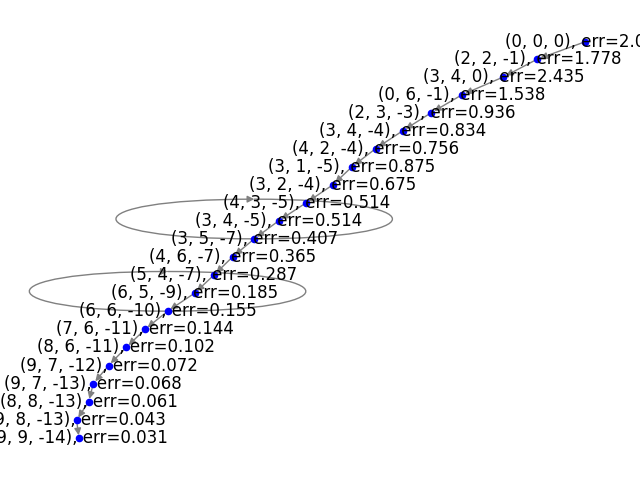
\includegraphics[width=6in]{_static/Figure_3_Temp=1.2_Path=23.png}
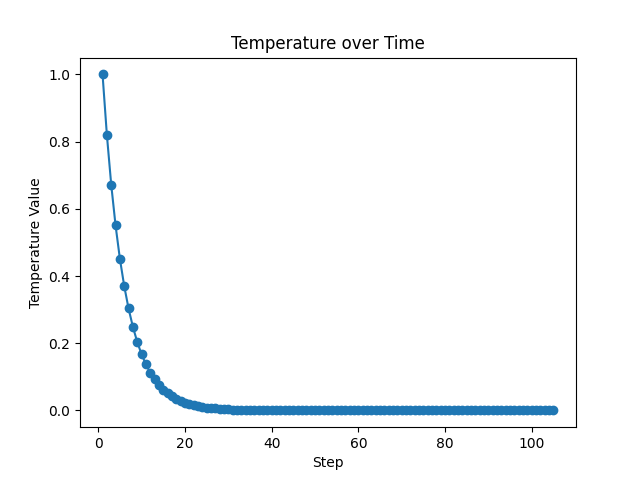
\includegraphics[width=6in]{_static/Figure_6_Temp=1.2_Temp-over-Time.png}
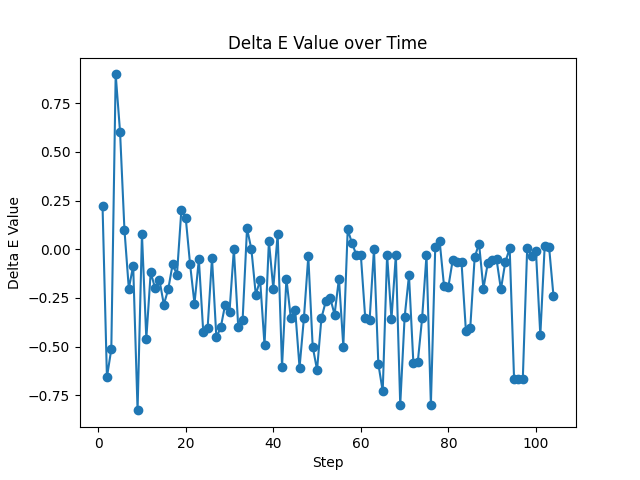
\includegraphics[width=6in]{_static/Figure_9_Temp=1.22_Delta-E-over-Time.png}
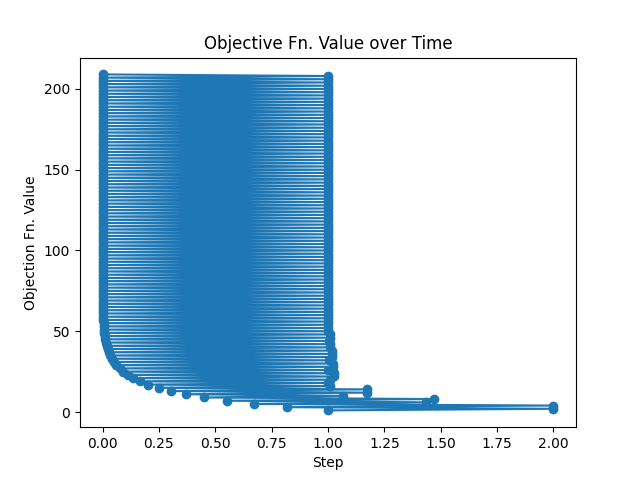
\includegraphics[width=6in]{_static/Figure_10_Temp=1.22_Obj-Fn-over-Time.png}

---

\subsection{Rapidly Cooling Schedule}

$$\lambda x : x / 5$$

This was a temperature schedule to see what an extreme change would do to the algorithm. 
It performed very poorly, failing to produce correct results in most runs.

However, the average traced search path length was significantly reduced:

\begin{itemize}
    \item for subpar results $= 9$.
    \item for good results $= 5$
\end{itemize}

Cooling off more quickly can speed up the search, but at the cost of accuracy.

See the $x : x / 5$ output graph:

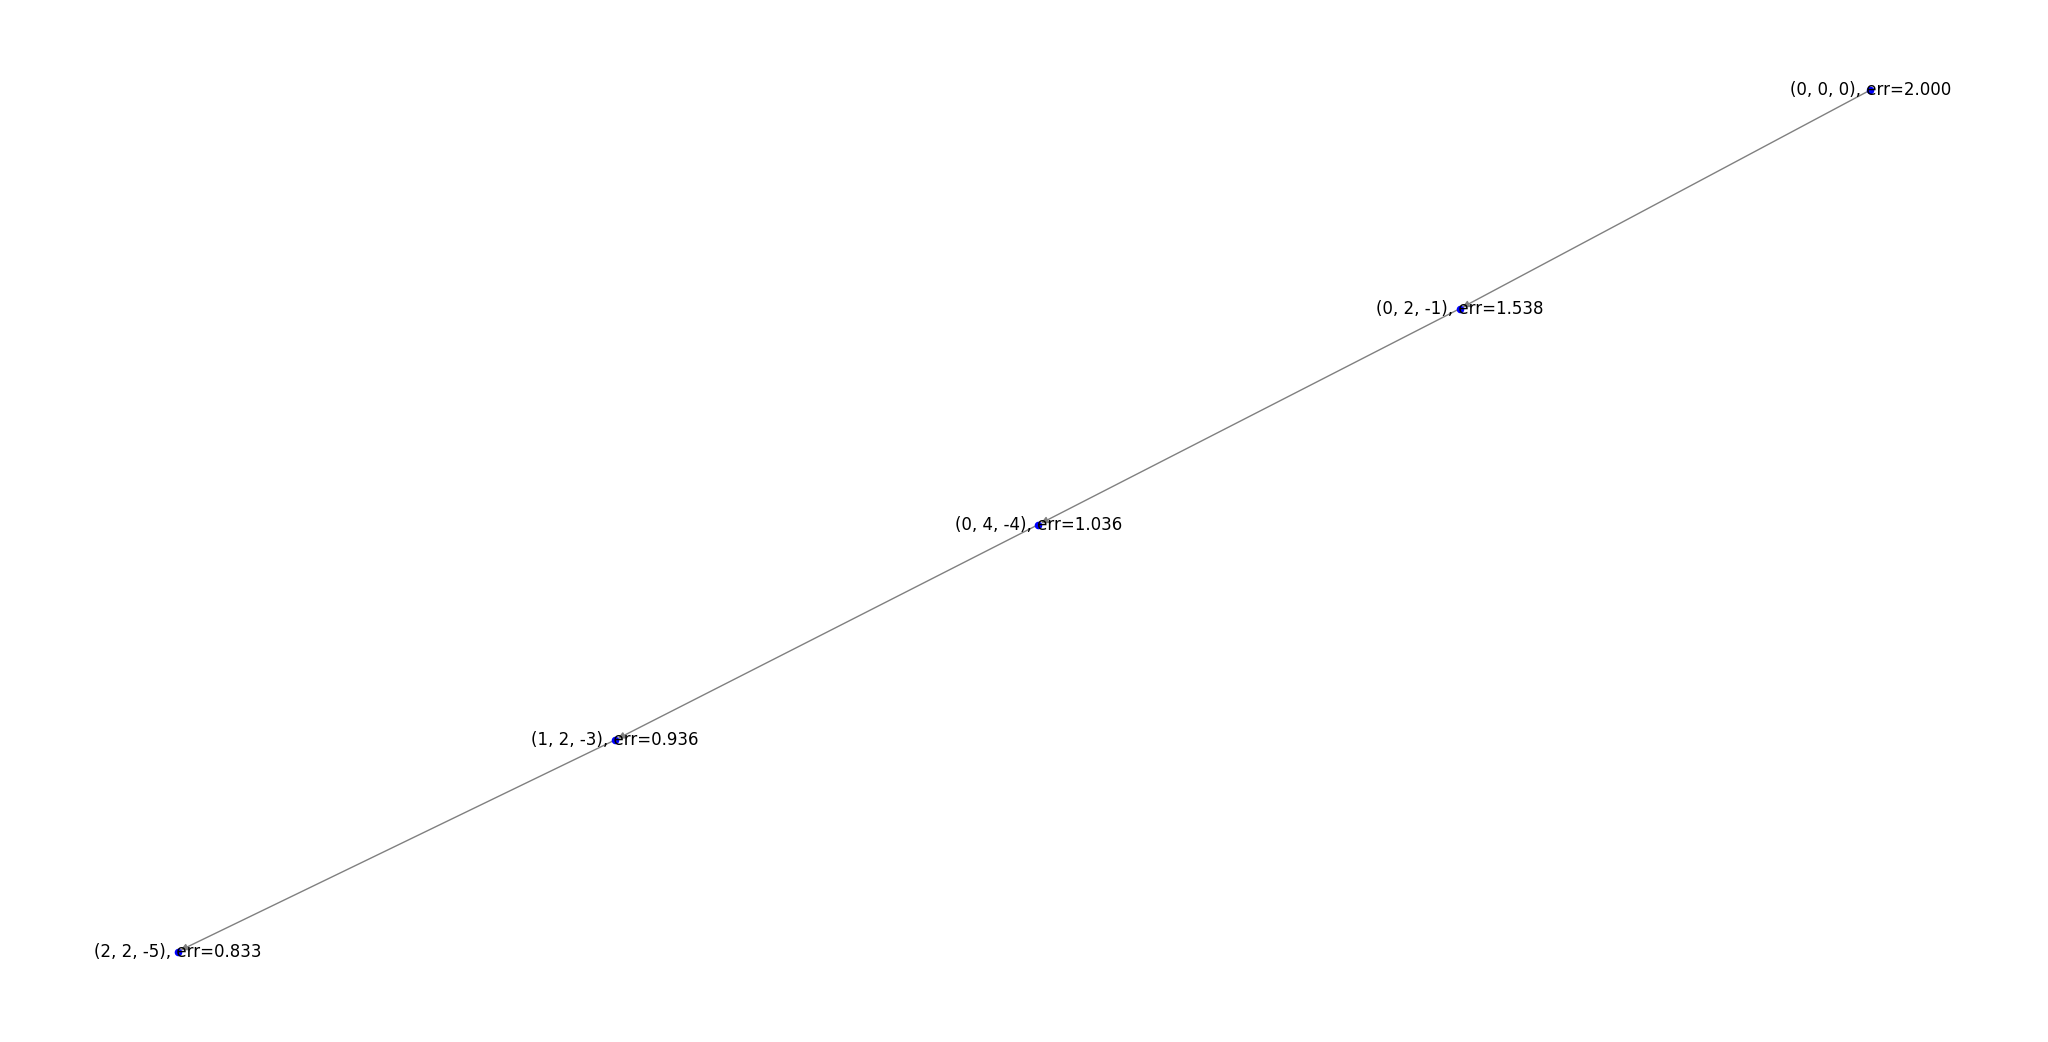
\includegraphics[width=6in]{_static/Figure_4_Temp=5_Path=5.png}
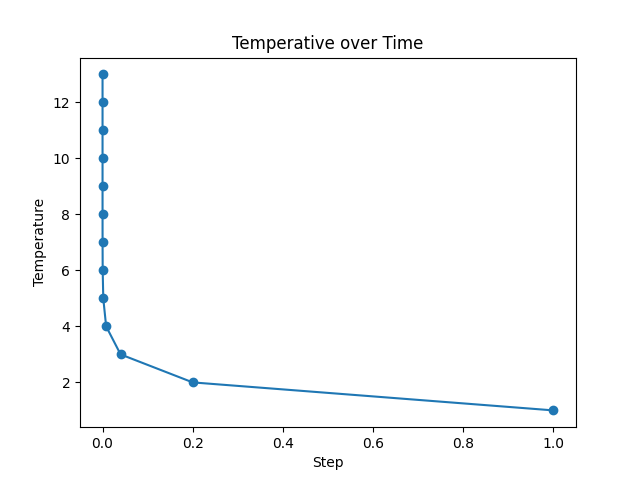
\includegraphics[width=6in]{_static/Figure_7_Temp=5_Temp-over-Time.png}

---

\subsection{Simmering Schedule}

$$\lambda x : x / 1.02$$

Now shifting to the opposite end of the spectrum by slowing down the rate of cooling.
It performed the worse, failing to ever produce correct results 
likely due to the extremely small $\Delta X$ causing near random-walk behavior.

Additionally, the average traced search path length was excessive:

\begin{itemize}
    \item for subpar results $> 1,000$.
    \item good results never happened.
\end{itemize}

Cooling off too quickly can slow down the search significantly 
and lead to unpredictable behavior.

See the $x : x / 1.02$ output graph:

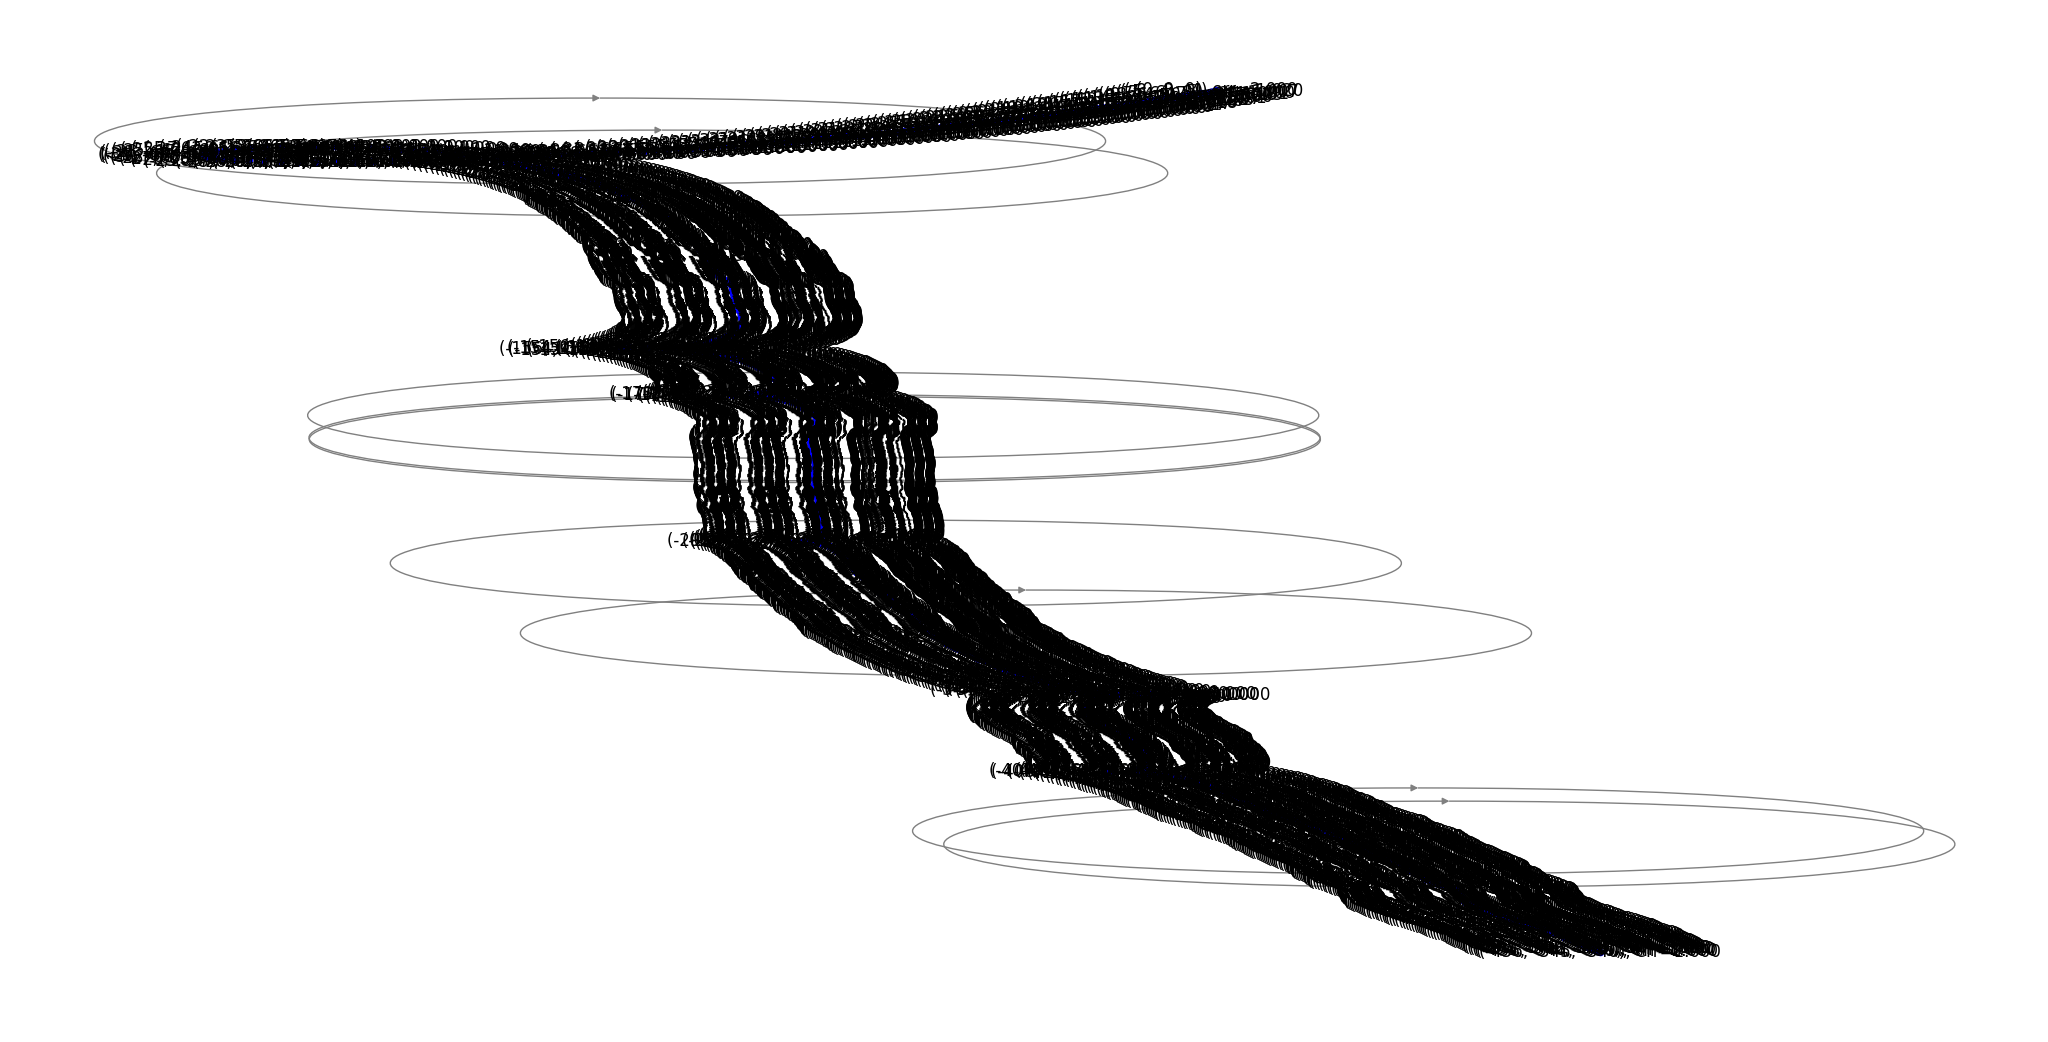
\includegraphics[width=6in]{_static/Figure_5_Temp=1.02_Path=1031.png}
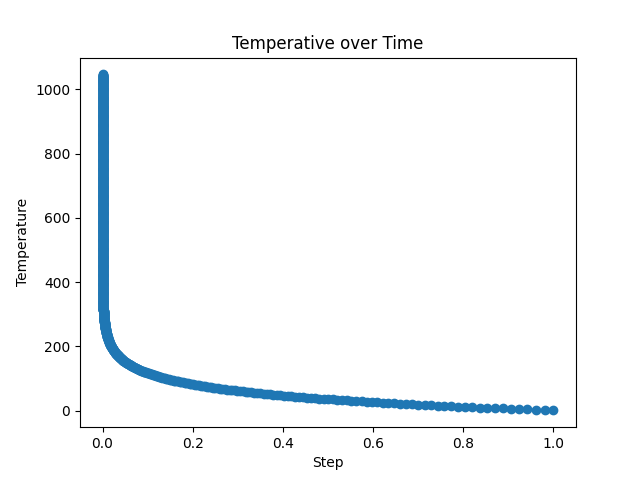
\includegraphics[width=6in]{_static/Figure_8_Temp=1.02_Temp-over-Time.png}

\section{Struggles}

\subsection{Learning Jupyter}

Learning what Jupyter notebook was and getting it to run took a good chunk of 
time out of working on my project. I also had to refactor my entire codebase 
to get it running in Jupyter notebook.

\subsection{Converting Report to LaTeX}

Converting this report to LateX from Markdown as I orginally wrote it in 
seemed like a waste of time considering that GitHub markdown rendering can 
be very good.

\subsection{Tracing with the Spreadsheet}

I could explain the simulated annealing algorithm away, or I could trace it 
given a network graph, but I was unable to wrap my head around the spreadsheet 
tracing. The numbers kept changing which make the previous row's calculations 
incorrect for what shows in the cells.

\subsection{Data Modeling}

After a good amount of research, I decided to build on top of Python's built-in 
graphlib.TopologicalSorter.

Graphing done using pip packages networkx and matplotlib.

\section{Online Resources}

\begin{enumerate}
    \item GitHub repository: \url{https://github.com/ahester57/simulated_annealing}.
    \item Learn LaTeX: \url{https://www.overleaf.com/learn}.
    \item Python graphlib: \url{https://docs.python.org/3/library/graphlib.html#}.
    \item Python virtual environments: \url{https://docs.python.org/3/tutorial/venv.html}.
    \item Jupyter Notebook Coach: \url{https://chat.openai.com/g/g-QAzs1b7Si-jupyter-notebook-coach}.
    \item Markdown to LaTex: \url{https://chat.openai.com/g/g-eW4YzRIyC-note-converter}.
\end{enumerate}

\section{Example Output}

\begin{lstlisting}[language=bash, caption=Example Output of Program]
$ simulated_annealing -w DEBUG anneal
2024-02-28 21:07:45,470;WARNING;simulated_annealing;('nodes are in a cycle', [(-23, -30, -67), err=1.000, (-21, -32, -65), err=1.000, (-23, -30, -67), err=1.000])
2024-02-28 21:07:45,470;DEBUG;simulated_annealing;Static Order: cycle
2024-02-28 21:07:45,470;INFO;simulated_annealing;Winner: (-27, -30, -66), err=1.000
2024-02-28 21:07:45,471;INFO;simulated_annealing;Path Length: 113
2024-02-28 21:07:45,471;WARNING;simulated_annealing;Winner not good enough, restarting with attempt #3.
2024-02-28 21:07:45,471;DEBUG;simulated_annealing;initializing Neuron
2024-02-28 21:07:45,471;DEBUG;simulated_annealing;initializing ProblemGraph
2024-02-28 21:07:45,471;DEBUG;simulated_annealing;executing anneal command
2024-02-28 21:07:45,471;DEBUG;simulated_annealing;Initial: (0, 0, 0), err=2.000
2024-02-28 21:07:45,471;DEBUG;simulated_annealing;initializing Neuron
2024-02-28 21:07:45,471;DEBUG;simulated_annealing;-0.7243657277057198
2024-02-28 21:07:45,471;DEBUG;simulated_annealing;0.8333333333333334
2024-02-28 21:07:45,472;DEBUG;simulated_annealing;initializing Neuron
2024-02-28 21:07:45,472;DEBUG;simulated_annealing;0.4696492855901244
2024-02-28 21:07:45,472;DEBUG;simulated_annealing;Taking successor as better option (exploitation)
2024-02-28 21:07:45,472;DEBUG;simulated_annealing;initializing Neuron
2024-02-28 21:07:45,472;DEBUG;simulated_annealing;-0.007532128330114629
2024-02-28 21:07:45,472;DEBUG;simulated_annealing;0.5787037037037038
2024-02-28 21:07:45,472;DEBUG;simulated_annealing;Taking successor with probability 98% (exploration)
2024-02-28 21:07:45,472;DEBUG;simulated_annealing;initializing Neuron
2024-02-28 21:07:45,472;DEBUG;simulated_annealing;-0.9242343145200194
2024-02-28 21:07:45,472;DEBUG;simulated_annealing;0.48225308641975323
2024-02-28 21:07:45,472;DEBUG;simulated_annealing;initializing Neuron
2024-02-28 21:07:45,473;DEBUG;simulated_annealing;-0.842914235237892
2024-02-28 21:07:45,473;DEBUG;simulated_annealing;0.401877572016461
2024-02-28 21:07:45,473;DEBUG;simulated_annealing;initializing Neuron
2024-02-28 21:07:45,473;DEBUG;simulated_annealing;-0.6836327054524383
2024-02-28 21:07:45,473;DEBUG;simulated_annealing;0.3348979766803842
2024-02-28 21:07:45,473;DEBUG;simulated_annealing;Taking successor with probability 12% (exploration)
2024-02-28 21:07:45,473;DEBUG;simulated_annealing;initializing Neuron
2024-02-28 21:07:45,473;DEBUG;simulated_annealing;0.9831097041481931
2024-02-28 21:07:45,474;DEBUG;simulated_annealing;Taking successor as better option (exploitation)
2024-02-28 21:07:45,474;DEBUG;simulated_annealing;initializing Neuron
2024-02-28 21:07:45,474;DEBUG;simulated_annealing;0.30283562747455595
2024-02-28 21:07:45,474;DEBUG;simulated_annealing;Taking successor as better option (exploitation)
2024-02-28 21:07:45,474;DEBUG;simulated_annealing;initializing Neuron
2024-02-28 21:07:45,474;DEBUG;simulated_annealing;0.0
2024-02-28 21:07:45,474;DEBUG;simulated_annealing;0.19380669946781492
2024-02-28 21:07:45,474;DEBUG;simulated_annealing;Taking successor with probability 100% (exploration)
2024-02-28 21:07:45,475;DEBUG;simulated_annealing;initializing Neuron
2024-02-28 21:07:45,475;DEBUG;simulated_annealing;-0.22151554819242836
2024-02-28 21:07:45,475;DEBUG;simulated_annealing;0.1615055828898458
2024-02-28 21:07:45,475;DEBUG;simulated_annealing;initializing Neuron
2024-02-28 21:07:45,475;DEBUG;simulated_annealing;-0.4621171572600099
2024-02-28 21:07:45,475;DEBUG;simulated_annealing;0.13458798574153816
2024-02-28 21:07:45,475;DEBUG;simulated_annealing;initializing Neuron
2024-02-28 21:07:45,475;DEBUG;simulated_annealing;-0.23884734366457427
2024-02-28 21:07:45,476;DEBUG;simulated_annealing;0.11215665478461513
2024-02-28 21:07:45,476;DEBUG;simulated_annealing;initializing Neuron
2024-02-28 21:07:45,476;DEBUG;simulated_annealing;-0.4621171572600099
2024-02-28 21:07:45,476;DEBUG;simulated_annealing;0.09346387898717928
2024-02-28 21:07:45,476;DEBUG;simulated_annealing;initializing Neuron
2024-02-28 21:07:45,476;DEBUG;simulated_annealing;-0.22151554819242836
2024-02-28 21:07:45,476;DEBUG;simulated_annealing;0.07788656582264941
2024-02-28 21:07:45,477;DEBUG;simulated_annealing;initializing Neuron
2024-02-28 21:07:45,477;DEBUG;simulated_annealing;-0.3807970779778823
2024-02-28 21:07:45,477;DEBUG;simulated_annealing;0.06490547151887452
2024-02-28 21:07:45,477;DEBUG;simulated_annealing;initializing Neuron
2024-02-28 21:07:45,477;DEBUG;simulated_annealing;-0.15928152978545385
2024-02-28 21:07:45,477;DEBUG;simulated_annealing;0.05408789293239544
2024-02-28 21:07:45,477;DEBUG;simulated_annealing;initializing Neuron
2024-02-28 21:07:45,477;DEBUG;simulated_annealing;0.0
2024-02-28 21:07:45,478;DEBUG;simulated_annealing;0.045073244110329536
2024-02-28 21:07:45,478;DEBUG;simulated_annealing;Taking successor with probability 100% (exploration)
2024-02-28 21:07:45,478;DEBUG;simulated_annealing;initializing Neuron
2024-02-28 21:07:45,478;DEBUG;simulated_annealing;1.1102230246251565e-16
2024-02-28 21:07:45,478;DEBUG;simulated_annealing;Taking successor as better option (exploitation)
2024-02-28 21:07:45,478;DEBUG;simulated_annealing;initializing Neuron
2024-02-28 21:07:45,478;DEBUG;simulated_annealing;0.0
2024-02-28 21:07:45,478;DEBUG;simulated_annealing;0.031300863965506624
2024-02-28 21:07:45,479;DEBUG;simulated_annealing;Taking successor with probability 100% (exploration)
2024-02-28 21:07:45,479;DEBUG;simulated_annealing;initializing Neuron
2024-02-28 21:07:45,479;DEBUG;simulated_annealing;-1.1102230246251565e-16
2024-02-28 21:07:45,479;DEBUG;simulated_annealing;0.026084053304588854
2024-02-28 21:07:45,479;DEBUG;simulated_annealing;Taking successor with probability 99% (exploration)
2024-02-28 21:07:45,479;DEBUG;simulated_annealing;initializing Neuron
2024-02-28 21:07:45,479;DEBUG;simulated_annealing;0.10296704066025653
2024-02-28 21:07:45,479;DEBUG;simulated_annealing;Taking successor as better option (exploitation)
2024-02-28 21:07:45,480;DEBUG;simulated_annealing;initializing Neuron
2024-02-28 21:07:45,480;DEBUG;simulated_annealing;-0.2033692440147602
2024-02-28 21:07:45,480;DEBUG;simulated_annealing;0.018113925905964483
2024-02-28 21:07:45,480;DEBUG;simulated_annealing;initializing Neuron
2024-02-28 21:07:45,480;DEBUG;simulated_annealing;-0.18078252593914657
2024-02-28 21:07:45,480;DEBUG;simulated_annealing;0.015094938254970403
2024-02-28 21:07:45,480;DEBUG;simulated_annealing;initializing Neuron
2024-02-28 21:07:45,480;DEBUG;simulated_annealing;-0.13426770395598053
2024-02-28 21:07:45,480;DEBUG;simulated_annealing;0.012579115212475336
2024-02-28 21:07:45,480;DEBUG;simulated_annealing;initializing Neuron
2024-02-28 21:07:45,480;DEBUG;simulated_annealing;-0.1626362217614783
2024-02-28 21:07:45,480;DEBUG;simulated_annealing;0.010482596010396113
2024-02-28 21:07:45,482;DEBUG;simulated_annealing;initializing Neuron
2024-02-28 21:07:45,482;DEBUG;simulated_annealing;-0.17234207040384641
2024-02-28 21:07:45,482;DEBUG;simulated_annealing;0.008735496675330095
2024-02-28 21:07:45,482;DEBUG;simulated_annealing;initializing Neuron
2024-02-28 21:07:45,482;DEBUG;simulated_annealing;0.23527880639765497
2024-02-28 21:07:45,482;DEBUG;simulated_annealing;Taking successor as better option (exploitation)
2024-02-28 21:07:45,482;DEBUG;simulated_annealing;initializing Neuron
2024-02-28 21:07:45,483;DEBUG;simulated_annealing;-0.39262867277529223
2024-02-28 21:07:45,483;DEBUG;simulated_annealing;0.0060663171356459
2024-02-28 21:07:45,483;DEBUG;simulated_annealing;initializing Neuron
2024-02-28 21:07:45,483;DEBUG;simulated_annealing;-0.37661964162379225
2024-02-28 21:07:45,483;DEBUG;simulated_annealing;0.005055264279704917
2024-02-28 21:07:45,483;DEBUG;simulated_annealing;initializing Neuron
2024-02-28 21:07:45,483;DEBUG;simulated_annealing;-0.26210260522127404
2024-02-28 21:07:45,483;DEBUG;simulated_annealing;0.004212720233087431
2024-02-28 21:07:45,484;DEBUG;simulated_annealing;initializing Neuron
2024-02-28 21:07:45,484;DEBUG;simulated_annealing;-0.32191775154693214
2024-02-28 21:07:45,484;DEBUG;simulated_annealing;0.003510600194239526
2024-02-28 21:07:45,484;DEBUG;simulated_annealing;initializing Neuron
2024-02-28 21:07:45,484;DEBUG;simulated_annealing;-0.40183907707161726
2024-02-28 21:07:45,484;DEBUG;simulated_annealing;0.002925500161866272
2024-02-28 21:07:45,484;DEBUG;simulated_annealing;initializing Neuron
2024-02-28 21:07:45,485;DEBUG;simulated_annealing;0.15928152978545385
2024-02-28 21:07:45,485;DEBUG;simulated_annealing;Taking successor as better option (exploitation)
2024-02-28 21:07:45,485;DEBUG;simulated_annealing;initializing Neuron
2024-02-28 21:07:45,485;DEBUG;simulated_annealing;-0.49934558551005426
2024-02-28 21:07:45,485;DEBUG;simulated_annealing;0.002031597334629356
2024-02-28 21:07:45,485;DEBUG;simulated_annealing;initializing Neuron
2024-02-28 21:07:45,485;DEBUG;simulated_annealing;0.10335398508619442
2024-02-28 21:07:45,486;DEBUG;simulated_annealing;Taking successor as better option (exploitation)
2024-02-28 21:07:45,486;DEBUG;simulated_annealing;initializing Neuron
2024-02-28 21:07:45,486;DEBUG;simulated_annealing;-0.405580595939507
2024-02-28 21:07:45,486;DEBUG;simulated_annealing;0.0014108314823814974
2024-02-28 21:07:45,486;DEBUG;simulated_annealing;initializing Neuron
2024-02-28 21:07:45,486;DEBUG;simulated_annealing;-0.07235274990848528
2024-02-28 21:07:45,486;DEBUG;simulated_annealing;0.001175692901984581
2024-02-28 21:07:45,486;DEBUG;simulated_annealing;initializing Neuron
2024-02-28 21:07:45,487;DEBUG;simulated_annealing;0.14995045490235762
2024-02-28 21:07:45,487;DEBUG;simulated_annealing;Taking successor as better option (exploitation)
2024-02-28 21:07:45,487;DEBUG;simulated_annealing;initializing Neuron
2024-02-28 21:07:45,487;DEBUG;simulated_annealing;-0.32444377576500527
2024-02-28 21:07:45,487;DEBUG;simulated_annealing;0.0008164534041559592
2024-02-28 21:07:45,487;DEBUG;simulated_annealing;initializing Neuron
2024-02-28 21:07:45,487;DEBUG;simulated_annealing;0.0
2024-02-28 21:07:45,487;DEBUG;simulated_annealing;0.0006803778367966327
2024-02-28 21:07:45,488;DEBUG;simulated_annealing;Taking successor with probability 100% (exploration)
2024-02-28 21:07:45,488;DEBUG;simulated_annealing;initializing Neuron
2024-02-28 21:07:45,488;DEBUG;simulated_annealing;-0.12029883613240247
2024-02-28 21:07:45,488;DEBUG;simulated_annealing;0.0005669815306638605
2024-02-28 21:07:45,488;DEBUG;simulated_annealing;initializing Neuron
2024-02-28 21:07:45,488;DEBUG;simulated_annealing;-0.21043414470910185
2024-02-28 21:07:45,488;DEBUG;simulated_annealing;0.00047248460888655046
2024-02-28 21:07:45,488;DEBUG;simulated_annealing;initializing Neuron
2024-02-28 21:07:45,488;DEBUG;simulated_annealing;-0.14995045490235762
2024-02-28 21:07:45,488;DEBUG;simulated_annealing;0.0003937371740721254
2024-02-28 21:07:45,488;DEBUG;simulated_annealing;initializing Neuron
2024-02-28 21:07:45,489;DEBUG;simulated_annealing;-0.20600196138697172
2024-02-28 21:07:45,489;DEBUG;simulated_annealing;0.00032811431172677114
2024-02-28 21:07:45,489;DEBUG;simulated_annealing;initializing Neuron
2024-02-28 21:07:45,489;DEBUG;simulated_annealing;-0.7706604017936203
2024-02-28 21:07:45,489;DEBUG;simulated_annealing;0.00027342859310564265
2024-02-28 21:07:45,489;DEBUG;simulated_annealing;initializing Neuron
2024-02-28 21:07:45,489;DEBUG;simulated_annealing;-0.21043414470910185
2024-02-28 21:07:45,489;DEBUG;simulated_annealing;0.00022785716092136888
2024-02-28 21:07:45,490;DEBUG;simulated_annealing;initializing Neuron
2024-02-28 21:07:45,490;DEBUG;simulated_annealing;-0.701049322422092
2024-02-28 21:07:45,490;DEBUG;simulated_annealing;0.00018988096743447407
2024-02-28 21:07:45,490;DEBUG;simulated_annealing;initializing Neuron
2024-02-28 21:07:45,490;DEBUG;simulated_annealing;-0.6994590540130035
2024-02-28 21:07:45,490;DEBUG;simulated_annealing;0.0001582341395287284
2024-02-28 21:07:45,490;DEBUG;simulated_annealing;initializing Neuron
2024-02-28 21:07:45,490;DEBUG;simulated_annealing;-0.701049322422092
2024-02-28 21:07:45,490;DEBUG;simulated_annealing;0.000131861782940607
2024-02-28 21:07:45,490;DEBUG;simulated_annealing;initializing Neuron
2024-02-28 21:07:45,490;DEBUG;simulated_annealing;-0.5598292753167986
2024-02-28 21:07:45,490;DEBUG;simulated_annealing;0.00010988481911717251
2024-02-28 21:07:45,492;DEBUG;simulated_annealing;initializing Neuron
2024-02-28 21:07:45,492;DEBUG;simulated_annealing;-0.5555310508418646
2024-02-28 21:07:45,492;DEBUG;simulated_annealing;9.157068259764377e-05
2024-02-28 21:07:45,492;DEBUG;simulated_annealing;initializing Neuron
2024-02-28 21:07:45,492;DEBUG;simulated_annealing;-0.3400640557246005
2024-02-28 21:07:45,492;DEBUG;simulated_annealing;7.630890216470315e-05
2024-02-28 21:07:45,492;DEBUG;simulated_annealing;initializing Neuron
2024-02-28 21:07:45,493;DEBUG;simulated_annealing;-0.14995045490235778
2024-02-28 21:07:45,493;DEBUG;simulated_annealing;6.35907518039193e-05
2024-02-28 21:07:45,493;DEBUG;simulated_annealing;initializing Neuron
2024-02-28 21:07:45,493;DEBUG;simulated_annealing;-0.3357658312496665
2024-02-28 21:07:45,493;DEBUG;simulated_annealing;5.299229316993275e-05
2024-02-28 21:07:45,493;DEBUG;simulated_annealing;initializing Neuron
2024-02-28 21:07:45,493;DEBUG;simulated_annealing;-0.6994590540130035
2024-02-28 21:07:45,494;DEBUG;simulated_annealing;4.4160244308277294e-05
2024-02-28 21:07:45,494;DEBUG;simulated_annealing;initializing Neuron
2024-02-28 21:07:45,494;DEBUG;simulated_annealing;-1.3877787807814457e-16
2024-02-28 21:07:45,494;DEBUG;simulated_annealing;3.680020359023108e-05
2024-02-28 21:07:45,494;DEBUG;simulated_annealing;Taking successor with probability 99% (exploration)
2024-02-28 21:07:45,494;DEBUG;simulated_annealing;initializing Neuron
2024-02-28 21:07:45,494;DEBUG;simulated_annealing;-0.060483689806744095
2024-02-28 21:07:45,494;DEBUG;simulated_annealing;3.0666836325192565e-05
2024-02-28 21:07:45,495;DEBUG;simulated_annealing;initializing Neuron
2024-02-28 21:07:45,495;DEBUG;simulated_annealing;0.011371355745090628
2024-02-28 21:07:45,495;DEBUG;simulated_annealing;Taking successor as better option (exploitation)
2024-02-28 21:07:45,495;DEBUG;simulated_annealing;initializing Neuron
2024-02-28 21:07:45,495;DEBUG;simulated_annealing;-0.36555024451770557
2024-02-28 21:07:45,495;DEBUG;simulated_annealing;2.129641411471706e-05
2024-02-28 21:07:45,495;DEBUG;simulated_annealing;initializing Neuron
2024-02-28 21:07:45,495;DEBUG;simulated_annealing;0.07180574529140546
2024-02-28 21:07:45,496;DEBUG;simulated_annealing;Taking successor as better option (exploitation)
2024-02-28 21:07:45,496;DEBUG;simulated_annealing;initializing Neuron
2024-02-28 21:07:45,496;DEBUG;simulated_annealing;-0.41676640556589406
2024-02-28 21:07:45,496;DEBUG;simulated_annealing;1.4789176468553517e-05
2024-02-28 21:07:45,496;DEBUG;simulated_annealing;initializing Neuron
2024-02-28 21:07:45,496;DEBUG;simulated_annealing;-0.011322055484661253
2024-02-28 21:07:45,496;DEBUG;simulated_annealing;1.2324313723794597e-05
2024-02-28 21:07:45,497;DEBUG;simulated_annealing;initializing Neuron
2024-02-28 21:07:45,497;DEBUG;simulated_annealing;-0.7818340573335352
2024-02-28 21:07:45,497;DEBUG;simulated_annealing;1.0270261436495497e-05
2024-02-28 21:07:45,497;DEBUG;simulated_annealing;initializing Neuron
2024-02-28 21:07:45,497;DEBUG;simulated_annealing;-0.41676640556589406
2024-02-28 21:07:45,497;DEBUG;simulated_annealing;8.558551197079582e-06
2024-02-28 21:07:45,497;DEBUG;simulated_annealing;initializing Neuron
2024-02-28 21:07:45,497;DEBUG;simulated_annealing;0.0
2024-02-28 21:07:45,497;DEBUG;simulated_annealing;7.132125997566319e-06
2024-02-28 21:07:45,498;DEBUG;simulated_annealing;Taking successor with probability 100% (exploration)
2024-02-28 21:07:45,498;DEBUG;simulated_annealing;initializing Neuron
2024-02-28 21:07:45,498;DEBUG;simulated_annealing;-0.1765517409242506
2024-02-28 21:07:45,498;DEBUG;simulated_annealing;5.9434383313052655e-06
2024-02-28 21:07:45,498;DEBUG;simulated_annealing;initializing Neuron
2024-02-28 21:07:45,498;DEBUG;simulated_annealing;-0.031033469344023124
2024-02-28 21:07:45,498;DEBUG;simulated_annealing;4.9528652760877216e-06
2024-02-28 21:07:45,499;DEBUG;simulated_annealing;initializing Neuron
2024-02-28 21:07:45,499;DEBUG;simulated_annealing;-0.031033469344023124
2024-02-28 21:07:45,499;DEBUG;simulated_annealing;4.127387730073101e-06
2024-02-28 21:07:45,499;DEBUG;simulated_annealing;initializing Neuron
2024-02-28 21:07:45,499;DEBUG;simulated_annealing;-0.031033469344023124
2024-02-28 21:07:45,499;DEBUG;simulated_annealing;3.439489775060918e-06
2024-02-28 21:07:45,499;DEBUG;simulated_annealing;initializing Neuron
2024-02-28 21:07:45,499;DEBUG;simulated_annealing;0.01814630417766827
2024-02-28 21:07:45,500;DEBUG;simulated_annealing;Taking successor as better option (exploitation)
2024-02-28 21:07:45,500;DEBUG;simulated_annealing;initializing Neuron
2024-02-28 21:07:45,500;DEBUG;simulated_annealing;-0.19047393348396455
2024-02-28 21:07:45,500;DEBUG;simulated_annealing;2.3885345660145265e-06
2024-02-28 21:07:45,500;DEBUG;simulated_annealing;initializing Neuron
2024-02-28 21:07:45,500;DEBUG;simulated_annealing;-0.1575088705459747
2024-02-28 21:07:45,500;DEBUG;simulated_annealing;1.9904454716787723e-06
2024-02-28 21:07:45,501;DEBUG;simulated_annealing;initializing Neuron
2024-02-28 21:07:45,501;DEBUG;simulated_annealing;-0.08995204946907373
2024-02-28 21:07:45,501;DEBUG;simulated_annealing;1.6587045597323104e-06
2024-02-28 21:07:45,501;DEBUG;simulated_annealing;initializing Neuron
2024-02-28 21:07:45,501;DEBUG;simulated_annealing;-0.044955661903737065
2024-02-28 21:07:45,501;DEBUG;simulated_annealing;1.3822537997769254e-06
2024-02-28 21:07:45,501;DEBUG;simulated_annealing;initializing Neuron
2024-02-28 21:07:45,502;DEBUG;simulated_annealing;-0.20442983217749164
2024-02-28 21:07:45,502;DEBUG;simulated_annealing;1.1518781664807712e-06
2024-02-28 21:07:45,502;DEBUG;simulated_annealing;initializing Neuron
2024-02-28 21:07:45,502;DEBUG;simulated_annealing;-0.08995204946907348
2024-02-28 21:07:45,503;DEBUG;simulated_annealing;9.598984720673093e-07
2024-02-28 21:07:45,503;DEBUG;simulated_annealing;initializing Neuron
2024-02-28 21:07:45,503;DEBUG;simulated_annealing;-0.19469804510191888
2024-02-28 21:07:45,503;DEBUG;simulated_annealing;7.999153933894245e-07
2024-02-28 21:07:45,503;DEBUG;simulated_annealing;initializing Neuron
2024-02-28 21:07:45,503;DEBUG;simulated_annealing;-0.044955661903737065
2024-02-28 21:07:45,503;DEBUG;simulated_annealing;6.665961611578537e-07
2024-02-28 21:07:45,504;DEBUG;simulated_annealing;initializing Neuron
2024-02-28 21:07:45,504;DEBUG;simulated_annealing;-0.20442983217749164
2024-02-28 21:07:45,504;DEBUG;simulated_annealing;5.554968009648782e-07
2024-02-28 21:07:45,504;DEBUG;simulated_annealing;initializing Neuron
2024-02-28 21:07:45,504;DEBUG;simulated_annealing;0.022601159173163625
2024-02-28 21:07:45,504;DEBUG;simulated_annealing;Taking successor as better option (exploitation)
2024-02-28 21:07:45,504;DEBUG;simulated_annealing;initializing Neuron
2024-02-28 21:07:45,504;DEBUG;simulated_annealing;-0.2157337484625442
2024-02-28 21:07:45,505;DEBUG;simulated_annealing;3.8576166733672095e-07
2024-02-28 21:07:45,505;DEBUG;simulated_annealing;initializing Neuron
2024-02-28 21:07:45,505;DEBUG;simulated_annealing;0.004221656563920262
2024-02-28 21:07:45,505;DEBUG;simulated_annealing;Taking successor as better option (exploitation)
2024-02-28 21:07:45,505;DEBUG;simulated_annealing;initializing Neuron
2024-02-28 21:07:45,505;DEBUG;simulated_annealing;-0.03917287908731803
2024-02-28 21:07:45,505;DEBUG;simulated_annealing;2.678900467616118e-07
2024-02-28 21:07:45,505;DEBUG;simulated_annealing;initializing Neuron
2024-02-28 21:07:45,506;DEBUG;simulated_annealing;-0.0675568210769007
2024-02-28 21:07:45,506;DEBUG;simulated_annealing;2.2324170563467652e-07
2024-02-28 21:07:45,506;DEBUG;simulated_annealing;initializing Neuron
2024-02-28 21:07:45,506;DEBUG;simulated_annealing;0.004220753393450849
2024-02-28 21:07:45,506;DEBUG;simulated_annealing;Taking successor as better option (exploitation)
2024-02-28 21:07:45,506;DEBUG;simulated_annealing;initializing Neuron
2024-02-28 21:07:45,506;DEBUG;simulated_annealing;0.0031234084273195073
2024-02-28 21:07:45,506;DEBUG;simulated_annealing;Taking successor as better option (exploitation)
2024-02-28 21:07:45,507;DEBUG;simulated_annealing;initializing Neuron
2024-02-28 21:07:45,507;DEBUG;simulated_annealing;-0.0015616430980205376
2024-02-28 21:07:45,507;DEBUG;simulated_annealing;1.291908018719193e-07
2024-02-28 21:07:45,507;DEBUG;simulated_annealing;initializing Neuron
2024-02-28 21:07:45,507;DEBUG;simulated_annealing;-0.07098936605674039
2024-02-28 21:07:45,507;DEBUG;simulated_annealing;1.0765900155993276e-07
2024-02-28 21:07:45,507;DEBUG;simulated_annealing;initializing Neuron
2024-02-28 21:07:45,507;DEBUG;simulated_annealing;0.0
2024-02-28 21:07:45,508;DEBUG;simulated_annealing;8.97158346332773e-08
2024-02-28 21:07:45,508;DEBUG;simulated_annealing;Taking successor with probability 100% (exploration)
2024-02-28 21:07:45,508;DEBUG;simulated_annealing;initializing Neuron
2024-02-28 21:07:45,508;DEBUG;simulated_annealing;-0.6819013630044626
2024-02-28 21:07:45,508;DEBUG;simulated_annealing;7.476319552773109e-08
2024-02-28 21:07:45,508;DEBUG;simulated_annealing;initializing Neuron
2024-02-28 21:07:45,508;DEBUG;simulated_annealing;0.02787809125324117
2024-02-28 21:07:45,508;DEBUG;simulated_annealing;Taking successor as better option (exploitation)
2024-02-28 21:07:45,509;DEBUG;simulated_annealing;initializing Neuron
2024-02-28 21:07:45,509;DEBUG;simulated_annealing;-0.029439734351261706
2024-02-28 21:07:45,509;DEBUG;simulated_annealing;5.1918885783146595e-08
2024-02-28 21:07:45,509;DEBUG;simulated_annealing;initializing Neuron
2024-02-28 21:07:45,509;DEBUG;simulated_annealing;-0.24881800951752175
2024-02-28 21:07:45,509;DEBUG;simulated_annealing;4.326573815262216e-08
2024-02-28 21:07:45,509;DEBUG;simulated_annealing;initializing Neuron
2024-02-28 21:07:45,510;DEBUG;simulated_annealing;-0.09886745730998155
2024-02-28 21:07:45,510;DEBUG;simulated_annealing;3.6054781793851806e-08
2024-02-28 21:07:45,510;DEBUG;simulated_annealing;initializing Neuron
2024-02-28 21:07:45,510;DEBUG;simulated_annealing;-0.09850371180052737
2024-02-28 21:07:45,510;DEBUG;simulated_annealing;3.0045651494876506e-08
2024-02-28 21:07:45,510;DEBUG;simulated_annealing;initializing Neuron
2024-02-28 21:07:45,510;DEBUG;simulated_annealing;-0.029439734351261706
2024-02-28 21:07:45,510;DEBUG;simulated_annealing;2.503804291239709e-08
2024-02-28 21:07:45,511;DEBUG;simulated_annealing;initializing Neuron
2024-02-28 21:07:45,511;DEBUG;simulated_annealing;-0.1004290554416117
2024-02-28 21:07:45,511;DEBUG;simulated_annealing;2.086503576033091e-08
2024-02-28 21:07:45,511;DEBUG;simulated_annealing;initializing Neuron
2024-02-28 21:07:45,511;DEBUG;simulated_annealing;-0.09850371180052737
2024-02-28 21:07:45,511;DEBUG;simulated_annealing;1.7387529800275758e-08
2024-02-28 21:07:45,511;DEBUG;simulated_annealing;initializing Neuron
2024-02-28 21:07:45,511;DEBUG;simulated_annealing;-0.09850371180052737
2024-02-28 21:07:45,511;DEBUG;simulated_annealing;1.4489608166896465e-08
2024-02-28 21:07:45,511;DEBUG;simulated_annealing;initializing Neuron
2024-02-28 21:07:45,511;DEBUG;simulated_annealing;-0.10035103256493168
2024-02-28 21:07:45,511;DEBUG;simulated_annealing;1.2074673472413721e-08
2024-02-28 21:07:45,512;DEBUG;simulated_annealing;initializing Neuron
2024-02-28 21:07:45,512;DEBUG;simulated_annealing;-0.47879887233498275
2024-02-28 21:07:45,512;DEBUG;simulated_annealing;1.0062227893678101e-08
2024-02-28 21:07:45,512;DEBUG;simulated_annealing;initializing Neuron
2024-02-28 21:07:45,512;DEBUG;simulated_annealing;-0.09829174661886426
2024-02-28 21:07:45,512;DEBUG;simulated_annealing;8.385189911398418e-09
2024-02-28 21:07:45,513;DEBUG;simulated_annealing;initializing Neuron
2024-02-28 21:07:45,513;DEBUG;simulated_annealing;0.0055114881721360955
2024-02-28 21:07:45,513;DEBUG;simulated_annealing;Taking successor as better option (exploitation)
2024-02-28 21:07:45,513;DEBUG;simulated_annealing;initializing Neuron
2024-02-28 21:07:45,513;DEBUG;simulated_annealing;-0.009731787075572686
2024-02-28 21:07:45,513;DEBUG;simulated_annealing;5.823048549582235e-09
2024-02-28 21:07:45,513;DEBUG;simulated_annealing;initializing Neuron
2024-02-28 21:07:45,513;DEBUG;simulated_annealing;-0.009731787075572654
2024-02-28 21:07:45,513;DEBUG;simulated_annealing;4.852540457985196e-09
2024-02-28 21:07:45,514;DEBUG;simulated_annealing;initializing Neuron
2024-02-28 21:07:45,514;DEBUG;simulated_annealing;-0.253541743766061
2024-02-28 21:07:45,514;DEBUG;simulated_annealing;4.043783714987663e-09
2024-02-28 21:07:45,514;DEBUG;simulated_annealing;initializing Neuron
2024-02-28 21:07:45,514;DEBUG;simulated_annealing;-0.034163468599800934
2024-02-28 21:07:45,514;DEBUG;simulated_annealing;3.3698197624897198e-09
2024-02-28 21:07:45,514;DEBUG;simulated_annealing;initializing Neuron
2024-02-28 21:07:45,515;DEBUG;simulated_annealing;-0.009731787075572654
2024-02-28 21:07:45,515;DEBUG;simulated_annealing;2.8081831354081e-09
2024-02-28 21:07:45,515;DEBUG;simulated_annealing;initializing Neuron
2024-02-28 21:07:45,515;DEBUG;simulated_annealing;-0.03281385219204694
2024-02-28 21:07:45,515;DEBUG;simulated_annealing;2.3401526128400836e-09
2024-02-28 21:07:45,515;DEBUG;simulated_annealing;initializing Neuron
2024-02-28 21:07:45,515;DEBUG;simulated_annealing;-6.938893903907228e-18
2024-02-28 21:07:45,516;DEBUG;simulated_annealing;1.9501271773667363e-09
2024-02-28 21:07:45,516;DEBUG;simulated_annealing;Taking successor with probability 99% (exploration)
2024-02-28 21:07:45,516;DEBUG;simulated_annealing;initializing Neuron
2024-02-28 21:07:45,516;DEBUG;simulated_annealing;-0.009156014875851933
2024-02-28 21:07:45,516;DEBUG;simulated_annealing;1.625105981138947e-09
2024-02-28 21:07:45,516;DEBUG;simulated_annealing;initializing Neuron
2024-02-28 21:07:45,516;DEBUG;simulated_annealing;-0.25375372548993713
2024-02-28 21:07:45,516;DEBUG;simulated_annealing;1.354254984282456e-09
2024-02-28 21:07:45,517;DEBUG;simulated_annealing;initializing Neuron
2024-02-28 21:07:45,517;DEBUG;simulated_annealing;-0.009731787075572679
2024-02-28 21:07:45,517;DEBUG;simulated_annealing;1.12854582023538e-09
2024-02-28 21:07:45,517;WARNING;simulated_annealing;('nodes are in a cycle', [(2, 1, -3), err=0.936, (2, 1, -3), err=0.936])
2024-02-28 21:07:45,517;DEBUG;simulated_annealing;Static Order: cycle
2024-02-28 21:07:45,517;INFO;simulated_annealing;Winner: (10, 11, -16), err=0.016
2024-02-28 21:07:45,517;INFO;simulated_annealing;Path Length: 23
2024-02-28 21:07:45,517;INFO;simulated_annealing;Graph Length: 23
\end{lstlisting}

\section{The Code}

\begin{lstlisting}[language=Python, caption=Simulated Annealing Algorithm]
""" Implement the anneal command.

```
function SIMULATED-ANNEALING(problem, schedule) returns a solution State
  current <- problem.INITIAL
  for t = 1 to inf do
      T <- schedule(t)
      if T = 0 then return current
      next <- a randomly selected successor of current
      delta_E <- VALUE(current) - VALUE(next)
      if delta_E > 0 then current <- next
      else current <- next only with probability e^(-delta_E/T)
```

Stuart Russel, Peter Norvig. "Artificial Intelligence: A Modern Approach, 4th Edition" (2021)
"""
import numpy as np

from graphlib import CycleError
from typing import Callable

try:
    # for visual mode. `pip install -e .[visual]
    import matplotlib.pyplot as plt
    import networkx as nx
    DiGraph = nx.DiGraph
except ModuleNotFoundError:
    plt = None
    nx = None
    class DiGraph: pass

from ..core.logger import logger
from ..model.problem import ProblemGraph
from ..model.node import Neuron


def _anneal_step(
        problem:ProblemGraph,
        T:float,
        current:Neuron,
        successor:Neuron,
        G:DiGraph|None=None
    ) -> Neuron:
    """ Execute one step of the simulated annealing function.
    
    :param problem: The problem definition.
    :type problem: ProblemGraph
    :param T: Current temperature.
    :type T: float
    :param current: The current node, searching for a greener pasture.
    :type current: Neuron
    :param successor: One of the neighboring nodes, enticing.
    :type successor: Neuron
    :param G: The network graph, if visual mode enabled.
    :type G: networkx.DiGraph|None
    :return: Either the current or successor node
    :rtype: Neuron
    """
    delta_E = problem.evaluate_node(current) - problem.evaluate_node(successor)
    logger.debug(delta_E)
    if delta_E > 0:
        logger.debug("Taking successor as better option (exploitation)")
        problem.add(successor, current) # Trace the path
        if G is not None:
            G.add_edge(current, successor)
        return successor
    else:
        logger.debug(T)
        probability = np.exp(delta_E / T)
        if np.random.default_rng().uniform() < probability:
            logger.debug("Taking successor with probability %d%s (exploration)", probability*100, '%')
            problem.add(successor, current) # Trace the path
            if G is not None:
                G.add_edge(current, successor)
            return successor
    return current


def _anneal_loop(
        problem:ProblemGraph|None=None,
        schedule:Callable=lambda x : x / 1.2,
        G:DiGraph|None=None
    ) -> Neuron:
    """ Execute the simulated annealing algorithm.
    
    :param problem: The problem definition.
    :type problem: ProblemGraph
    :param schedule: Temperature function
    :type schedule: Callable
    :param G: The network graph, if visual mode enabled.
    :type G: networkx.DiGraph|None
    :return: The winner
    :rtype: Neuron
    """
    logger.debug("executing anneal command")
    assert isinstance(problem, ProblemGraph)
    assert isinstance(schedule, Callable)
    current = problem.initial
    logger.debug("Initial: %s", current)
    T = 1
    for t in range(10000000):
        T = schedule(T)
        if T < 0.000000001: break
        successor = Neuron(
            *current.weights
           + np.random.default_rng()
                .integers(
                    low=-2.-current.error,
                   # widen step size as error increases
                    high=2.+current.error,
                    size=Neuron.DIM_W)
        )
        current = _anneal_step(problem, T, current, successor, G)
    return current


def main(problem:ProblemGraph|None=None, schedule:Callable=lambda x : x / 1.2) -> ProblemGraph:
    """ Entrypoint to the simulated annealing algorithm.
    
    :param problem: The problem definition.
    :type problem: ProblemGraph
    :param schedule: Temperature function
    :type schedule: Callable
    :return: The problem with solution search graph.
    :rtype: ProblemGraph
    """
    logger.debug("executing anneal command")
    assert problem is None or isinstance(problem, ProblemGraph)
    assert schedule is None or isinstance(schedule, Callable)
    if problem is None:
        problem = ProblemGraph(Neuron(0, 0, 0))
    if schedule is None:
        schedule = lambda x : x / 1.2
    for attempt in range(1, 10):
        # Random Restarts 10x or until err < 0.5
        G = None
        if plt is not None and nx is not None:
            G = nx.DiGraph()
        # Run simulated annealing
        winner = _anneal_loop(problem, schedule, G)
        try:
            # Topological sort
            static_order = tuple(problem.static_order())
        except CycleError as cycerr:
            logger.warn(cycerr)
            static_order = 'cycle'
        logger.debug(f"Static Order: {static_order}")
        logger.info("Winner: %s", winner)
        logger.info("Path Length: %s", len(problem.graph.keys()))
        if winner.error < 0.5:
            break
        logger.warn("Winner not good enough, restarting with attempt #%d.", attempt)
        problem = ProblemGraph(Neuron(0, 0, 0))
    if G is not None:
        logger.info("Graph Length: %s", len(G))
        pos = nx.kamada_kawai_layout(G, weight=None)
        nx.draw(G, pos, with_labels=True, node_color='blue', edge_color='grey', node_size=20)
        plt.show()
    return problem


if __name__ == "__main__":
    main()

\end{lstlisting}

\section{Python Package Requirements}

\begin{lstlisting}[language=Toml, caption=Python Project Definition]
[build-system]
requires = ["setuptools>=61.0"]
build-backend = "setuptools.build_meta"

[project]
name = "simulated_annealing"
description = "A simulated annealing process to determine the optimal weight values of an artificial neuron."
authors = [
    { name = "Austin Hester", email = "ahester57@gmail.com" },
]
license = {file = "LICENSE"}
classifiers = [
    "Development Status :: 3 - Alpha",
    "Framework :: Pytest",
    "Intended Audience :: Education",
    "License :: OSI Approved :: MIT License",
    "Programming Language :: Python",
    "Programming Language :: Python :: 3",
    "Programming Language :: Python :: 3.8",
    "Programming Language :: Python :: 3.9",
    "Programming Language :: Python :: 3.10",
    "Programming Language :: Python :: 3.11",
    "Programming Language :: Python :: 3.12",
    "Natural Language :: English",
    "Topic :: Scientific/Engineering :: Artificial Intelligence",
    "Topic :: Education :: Testing"
]
requires-python = ">=3.8"
dependencies = [
    "numpy>=1.26.4,<2",
    "tomli==2.0.1; python_version<'3.11'",
]
dynamic = ["version", "readme"]

[project.urls]
"Homepage" = "https://github.com/ahester57/simulated_annealing"

[project.scripts]
simulated_annealing = "simulated_annealing.cli:main"

[project.optional-dependencies]
deep = [
    "keras>=3.0.5,<4",
    "torch>=2.1.2,<3",
    "torchvision>=0.16.2,<1",
]
dev = [
    "pytest>=7.3.1,<8",
    "sphinx>=6.2.1,<7",
    "sphinx_rtd_theme>=1.2.1,<2",
]
jupyter = [
    "notebook>=7.1.1,<8"
]
visual = [
    "networkx>=3.2.0,<4",
    "matplotlib>=3.8.3,<4",
    "scipy>=1.12.0,<2"
]

[tool.setuptools.dynamic]
version = {attr = "simulated_annealing.__version__"}
readme = {file = ["README.md"], content-type = "text/markdown"}

[tool.setuptools.packages.find]
where = ["src"]

\end{lstlisting}

\section{Further Documentation}
References to additional documentation within the repository.

\end{document}